\section{Lecture de plan}

On s'intéresse maintenant au motoréducteur donc les vues éclatées et écorchées sont présentées sur les figures \ref{fig11} et \ref{fig12}. La nomenclature est fournie en fin de sujet et un plan à compléter est fourni en document réponse.

\begin{figure}[ht!]
\begin{center}
    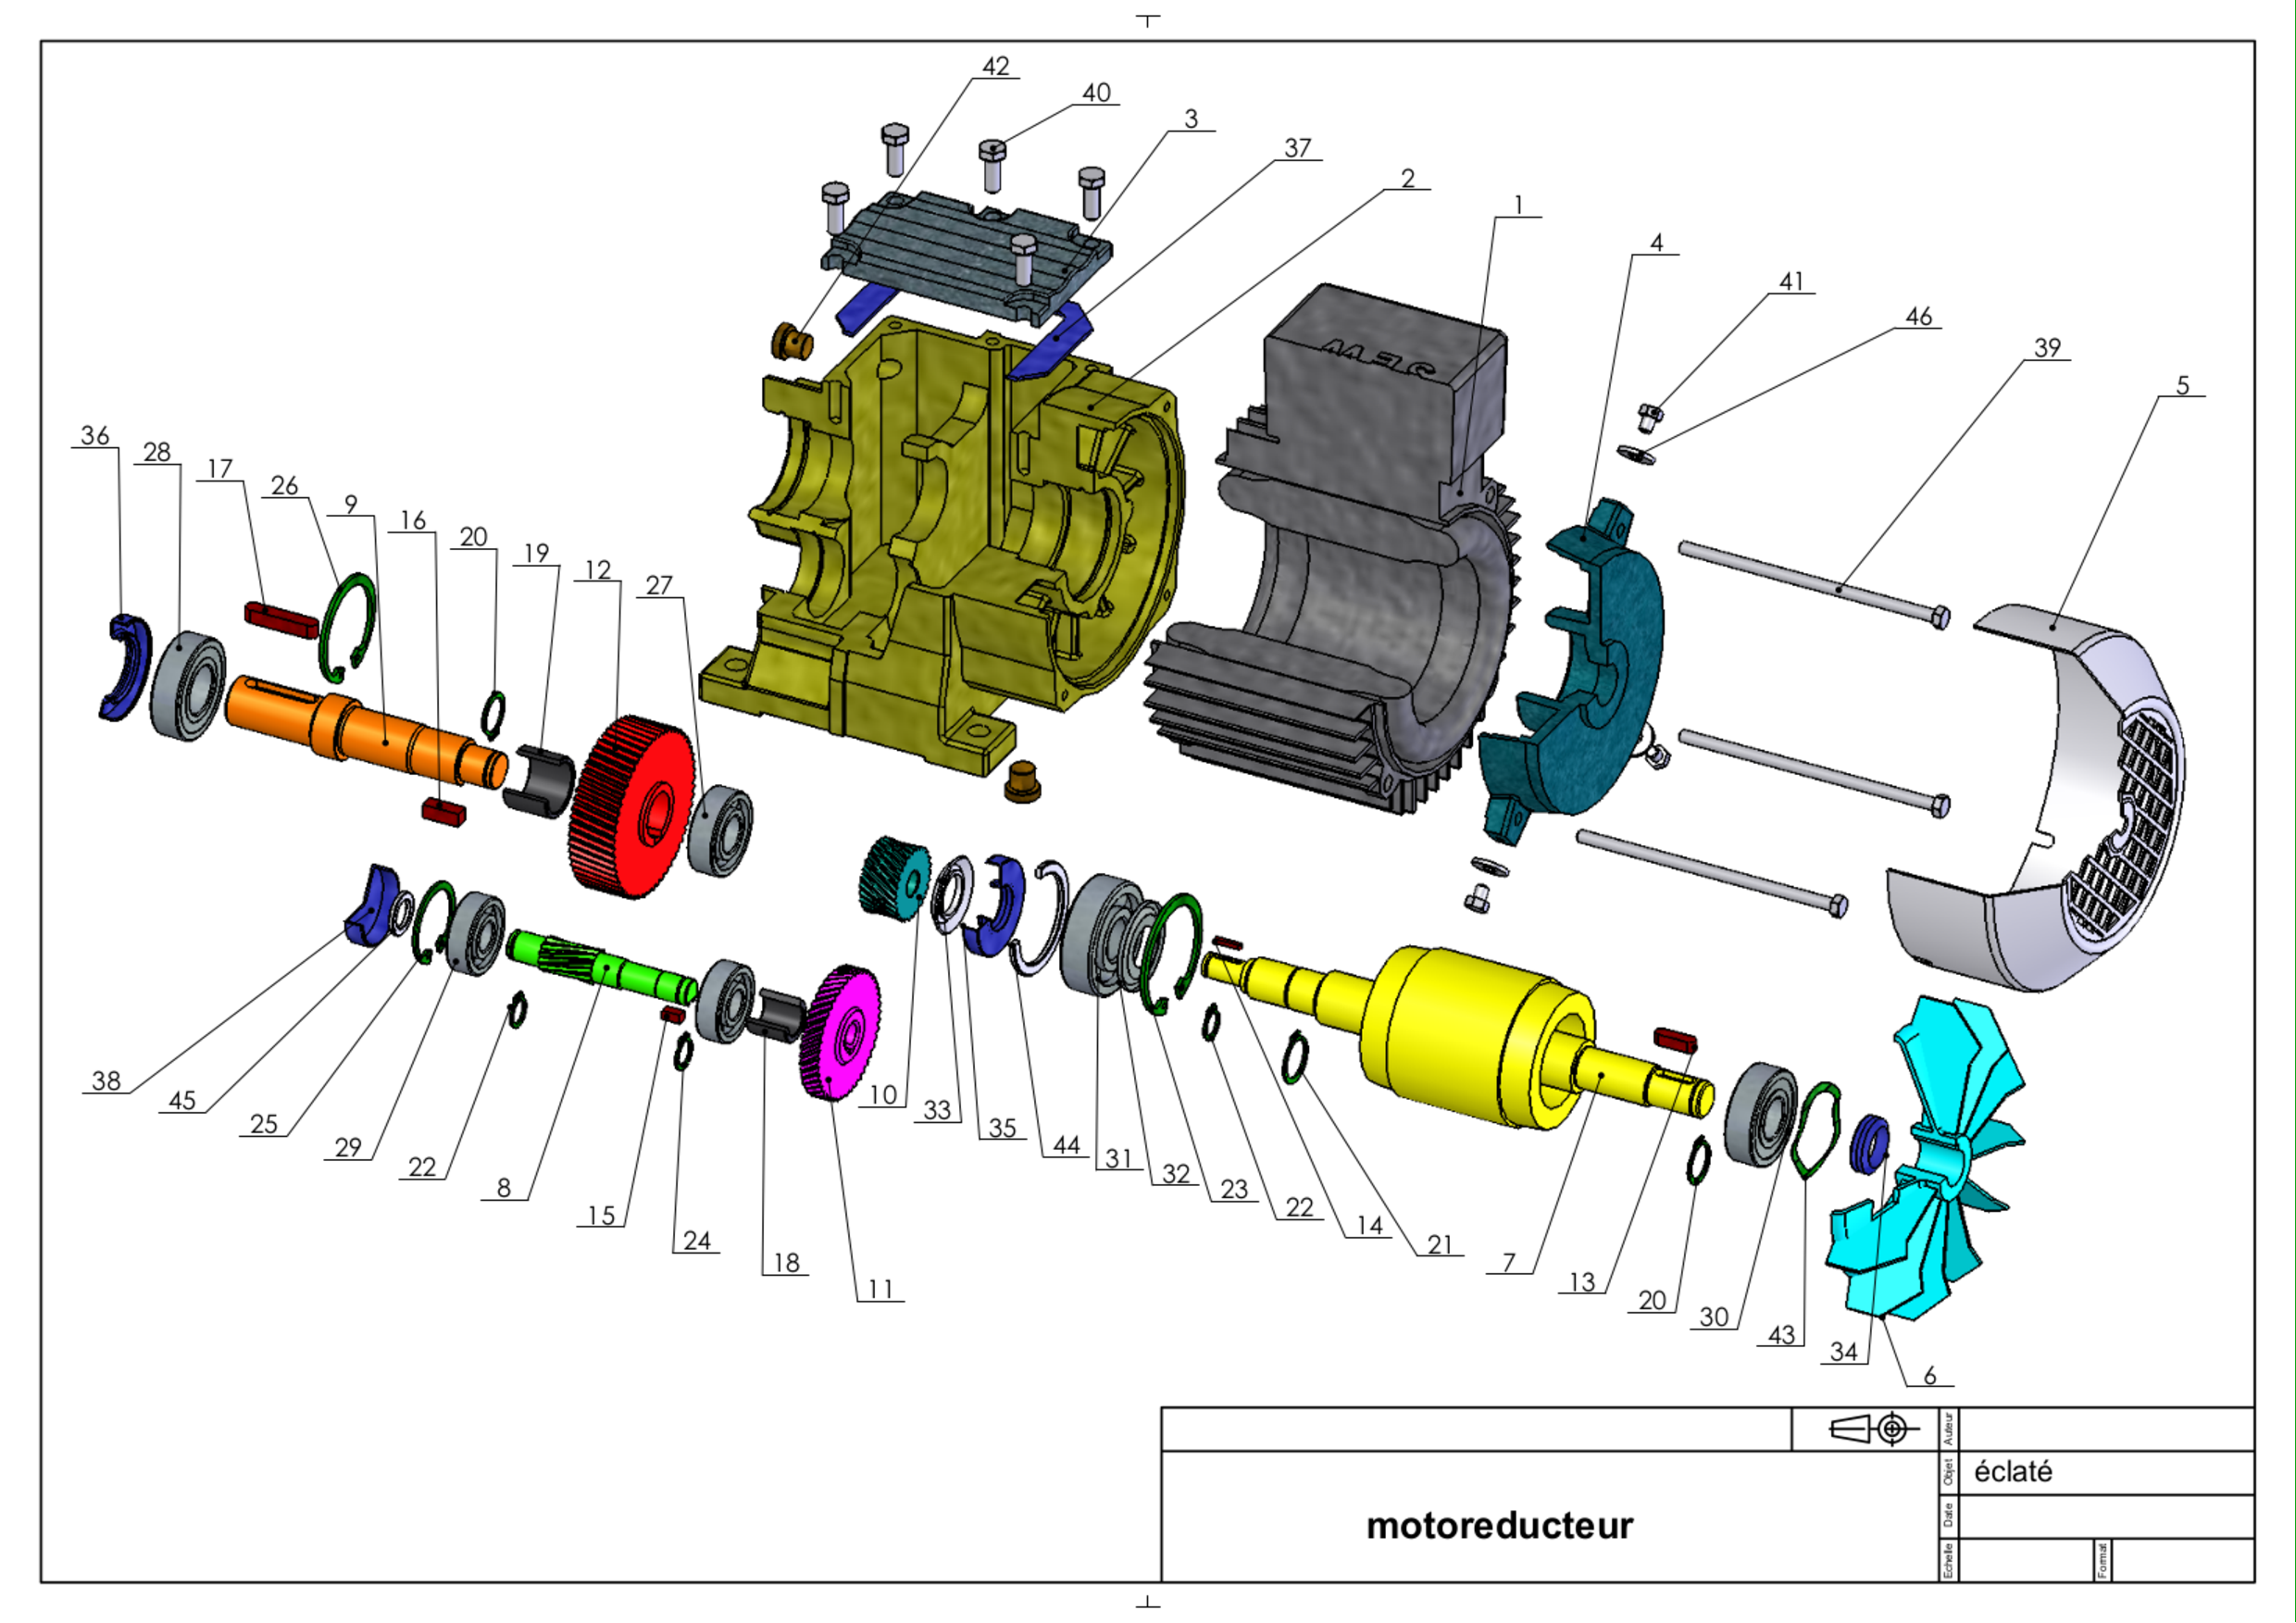
\includegraphics[width=0.75\linewidth]{img/eclate}
  \end{center}
    \caption{Vue éclatée du motoréducteur}
\label{fig11}
\end{figure}

\begin{figure}[ht!]
\begin{center}
    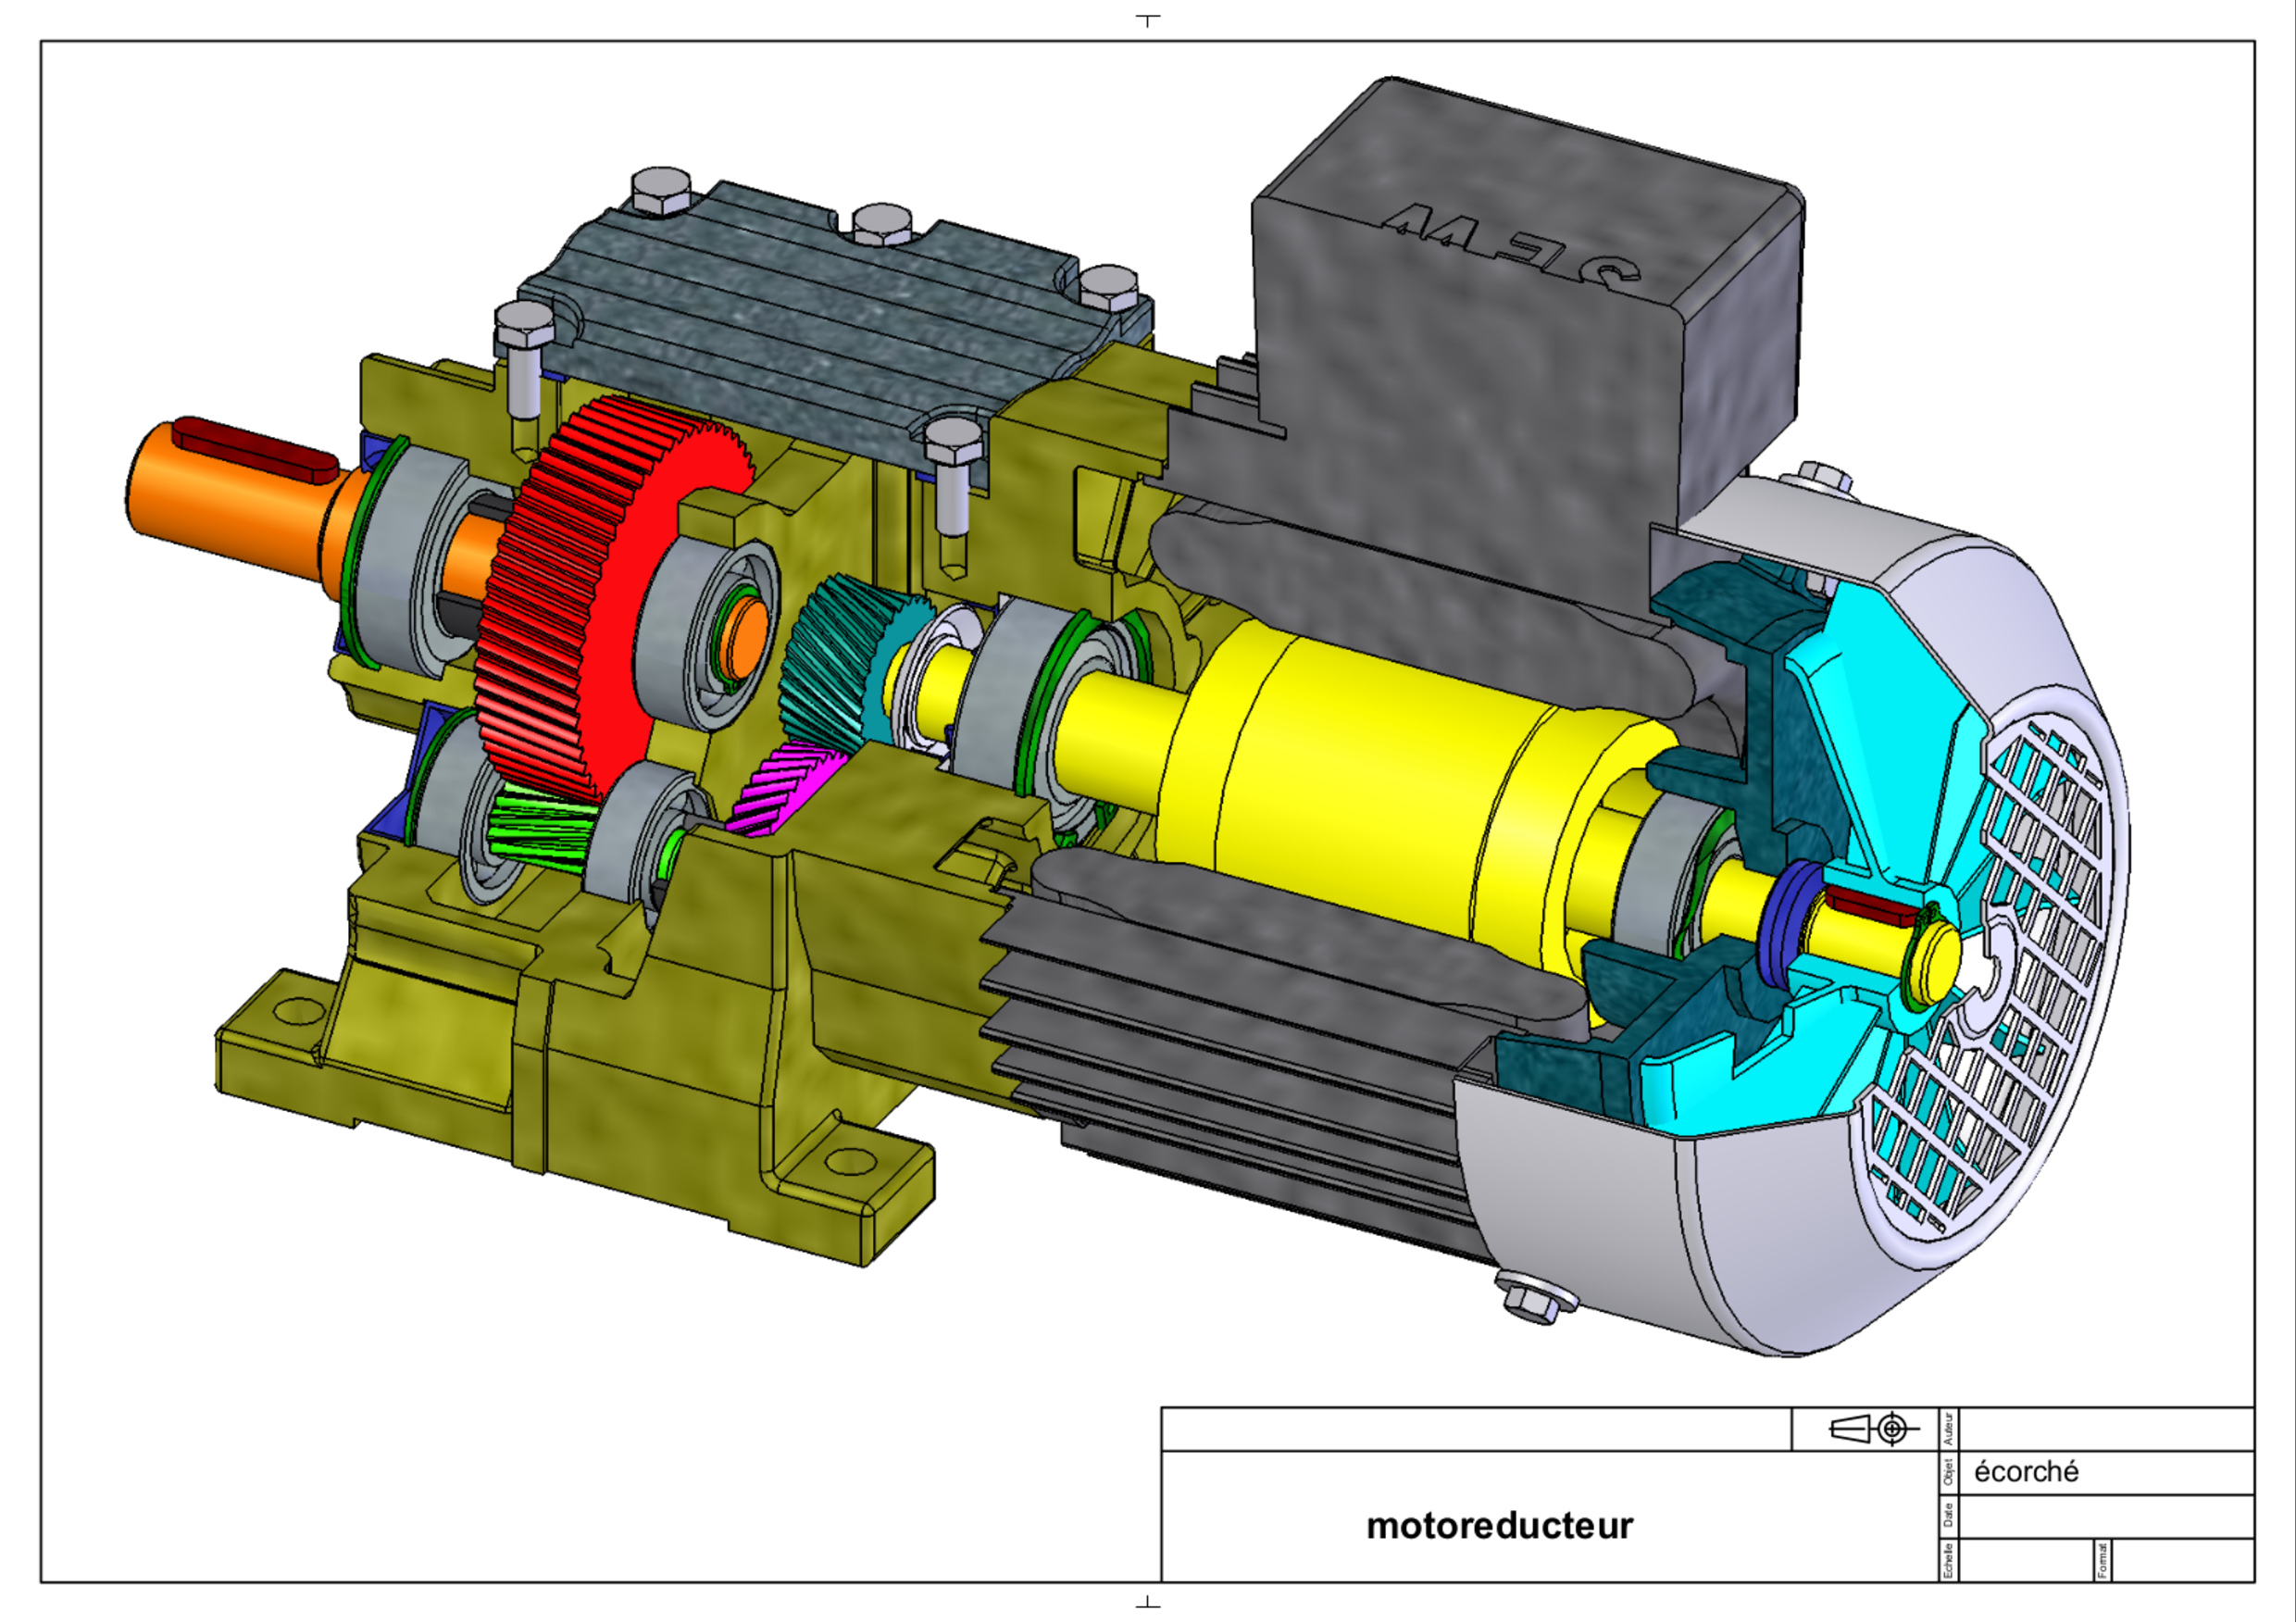
\includegraphics[width=0.75\linewidth]{img/ecorche}
  \end{center}
    \caption{Vue écorchée du motoréducteur}
\label{fig12}
\end{figure}

\question{Déterminer le rapport de réduction $\dfrac{\omega_{sortie}}{\omega_{rotor}}$.}

\question{A quoi correspond la pièce 6 ?}

\question{Colorier les classes d'équivalence du mécanisme (ne pas colorier à l'intérieur des ZONE 1 et ZONE 2).}

\question{Compléter la ZONE 1 en concevant une solution pour l'assemblage du pignon 10 avec le rotor 7. Vous pourrez utiliser la nomenclature afin de déterminer les pièces manquantes.}

\question{Compléter la ZONE 2 en concevant une solution pour l'assemblage du couvercle 3 sur le carter réducteur 2. Vous pourrez utiliser la nomenclature afin de déterminer les pièces manquantes.}

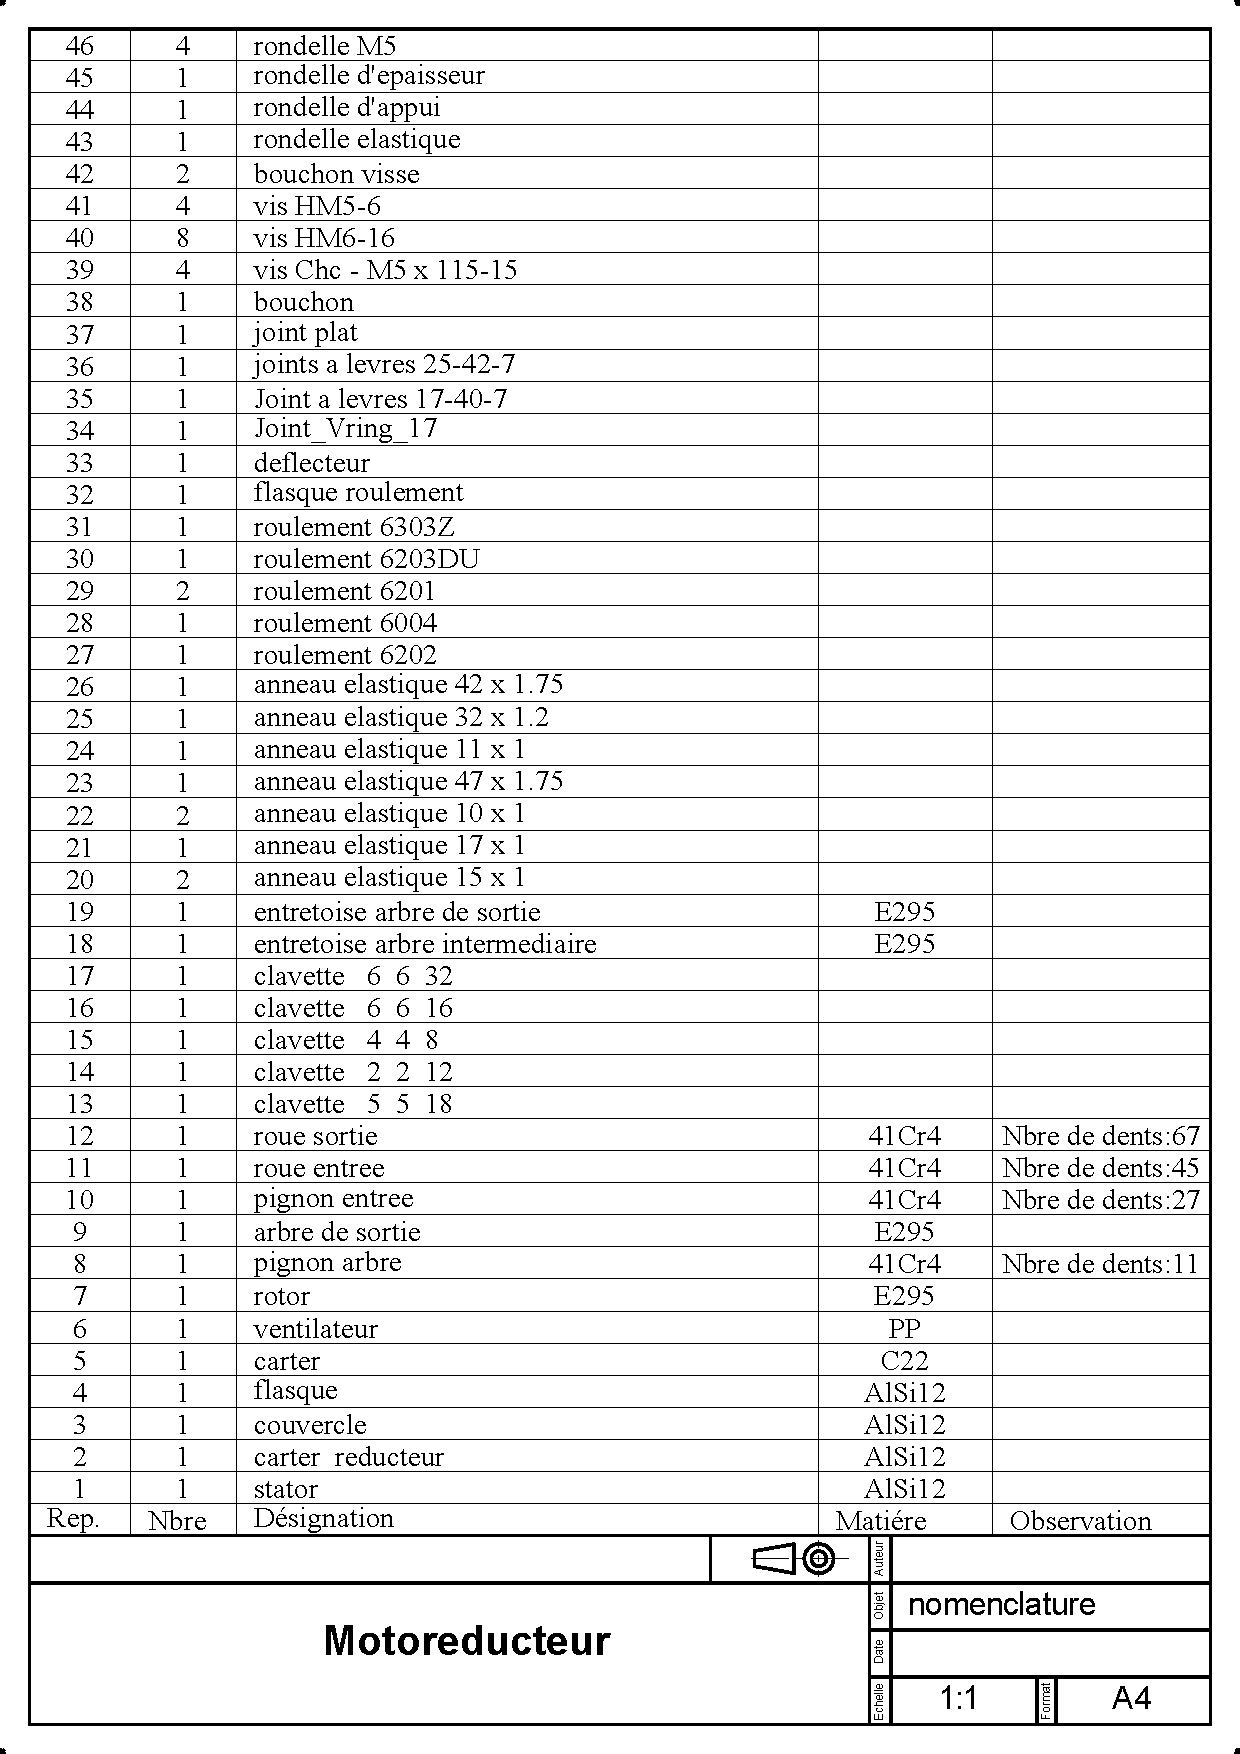
\includepdf[offset=-20 -20]{img/nomenclature.pdf}

\reponse{4}{}{$\dfrac{\omega_{sortie}}{\omega_{rotor}}=\dfrac{11.27}{45.67}=\dfrac{297}{2680+335}=\dfrac{297}{3015}\approx 0.1$}

\reponse{4}{}{Il est indiqué que c'est un ventilateur dans la nomenclature.}

\ifdef{\public}{}{

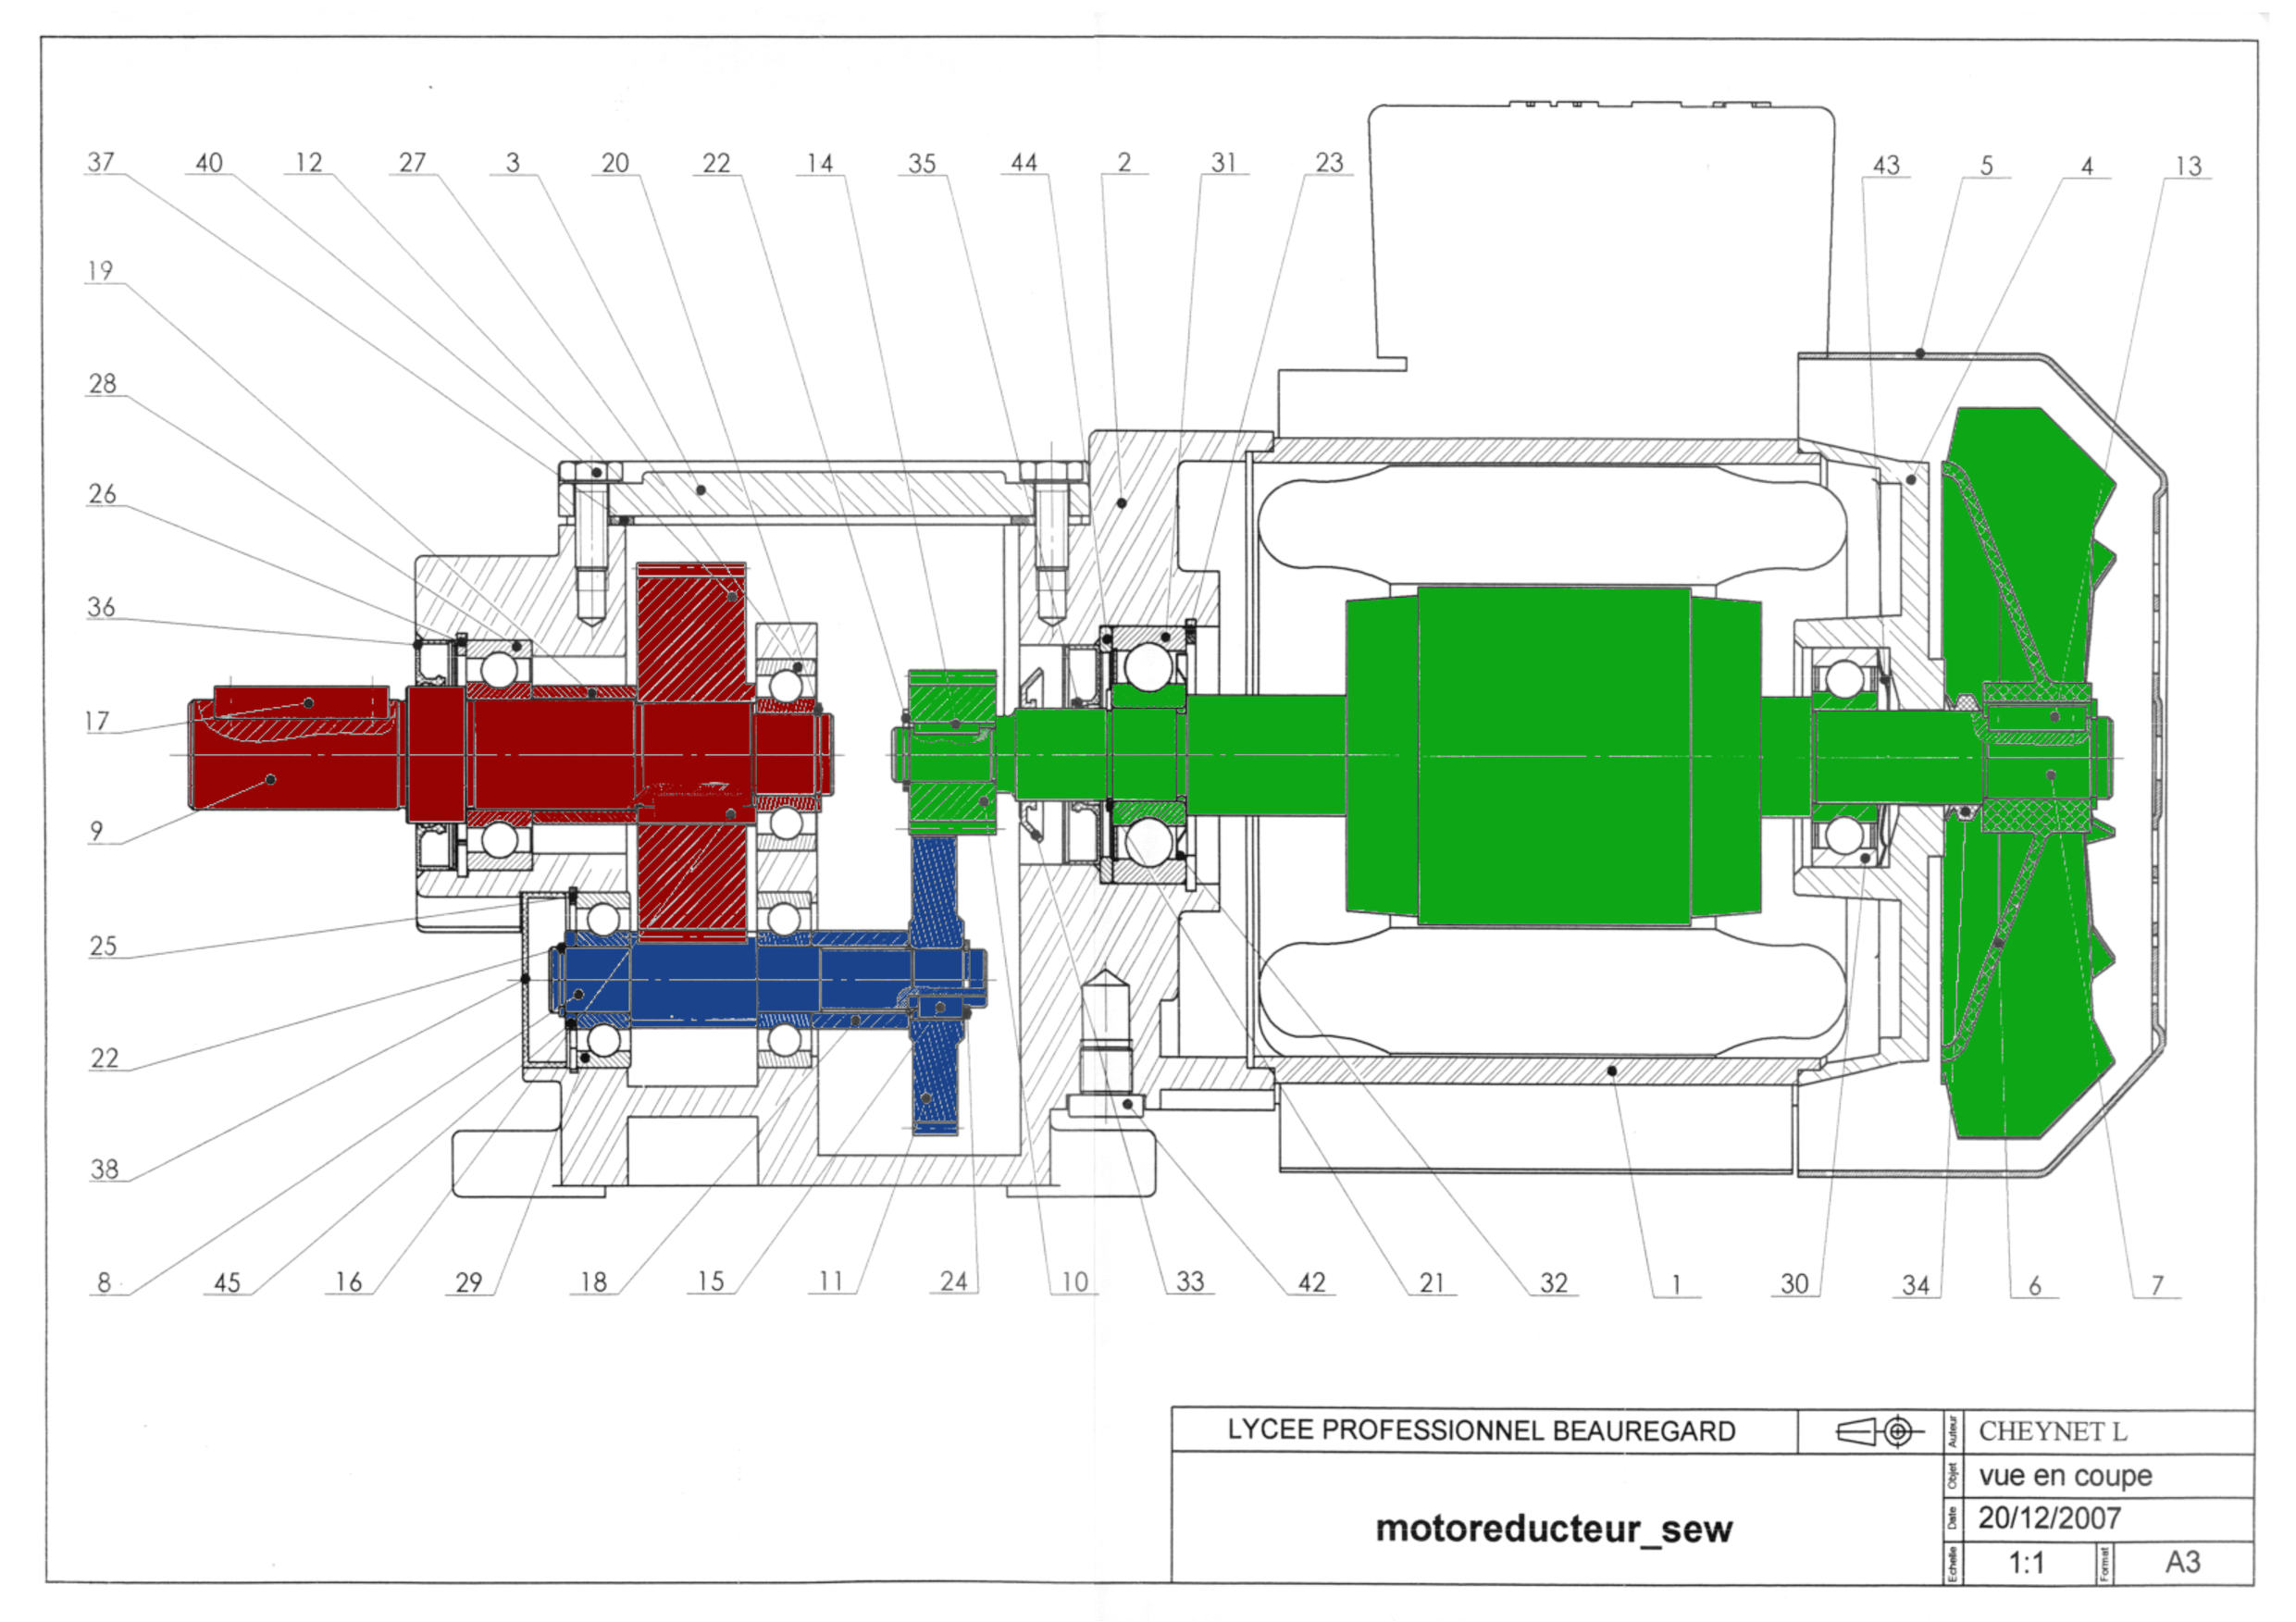
\includepdf[angle=90,offset=-20 -20]{img/Motoreducteur_classes_equivalence.pdf}

\includepdf[angle=90,offset=15 -20]{img/Motoreducteur_cor.pdf}
}
